\subsubsection{Minimising error}\label{minimizing-error}

Once one of the cost functions has been chosen, the aim is to minimise the error and thus improve the model:

\begin{equation}
\begin{split}
        W^* &= \argmin_{W} \frac{1}{n} \sum_{i=1}^n c(a(x^{(i)}; W), y^{(i)}) \\
        &= \argmin_{W} c_i(W) \\
        \text{where}~x^{(i)} &= \text{Input vector for data  }i \\
        y^{(i)} &= \text{Actual vector for data }i \\
        W &= \text{Matrices with the weights and biases of each} 
  \end{split}
\end{equation}

To calculate the minimum of a function, it is necessary to calculate the derivative of that function and equal it to $0$. Minimising the cost function, that is, deriving the cost function, also minimises the error. To do this there are different ways of minimising the error:

\begin{itemize}
\item \acrfull{ols}.

This was the algorithm used in the perceptron networks to calculate the $W$ matrix. Starting from the definition of any cost function that allows the quantification of the model error, an attempt will be made to minimise this value. One of the most popular equations is the one known as the \acrlong{ols}. This function is based on the \acrshort{mse} derivative:

\begin{equation}
    \begin{split}
    L_i & =  (\hat{y_i} - y_i)^2 \\
     & = (y - x \cdot W)' \cdot (y - x \cdot W) \\
     & = y'y - W'x'y - y'xW + W'x'x W
  \end{split}
\end{equation}

Deriving and clearing:
\begin{equation}
    \begin{split}
L_i'() = & -2x'y + 2x'xW \\
W^* = & (x'x)^{-1}x'y
\end{split}
\end{equation}


This equation allows the calculation of the optimal $W$-matrix possible only by using the model input and output values as arguments. Although this training algorithm has several limitations:
\begin{itemize}
\item It cannot be extended to more complex networks.
\item The calculation of the inverse matrix is very costly in terms of computation.
\item The minimum square error has been used, one of the simplest, since it is a function with a convex shape and therefore an easy derivative to calculate, but there are other cost functions that do not allow minimising the error with this technique.
\newline
\end{itemize}

These limitations, demonstrated mathematically in the book "\textit{Perceptron}" \cite{papert} by Minsky and Papert (1969), led to a sudden cut in funding for artificial intelligence projects and more specifically those related to neural network systems over a period of more than 15 years known as the winter of artificial intelligence.


\item Descending the gradient.

This algorithm is not a formula like \acrlong{ols}, but an iterative method that gradually minimizes error. Somehow it can be assimilated to how we human beings learn: Not with a single formula, but through experience reducing our errors over time.
\newline

The calculation of the gradient is a process that can be represented as follows:
\begin{figure}[H]
    \centering
    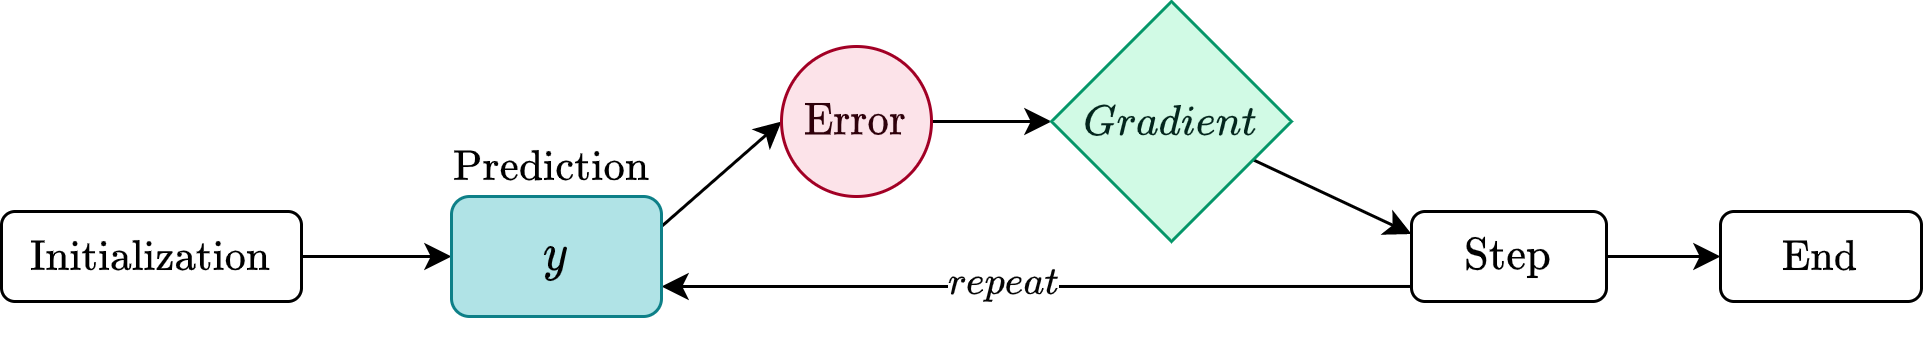
\includegraphics[width=13cm]{images/state-of-art/gradient-descent/gradient-algorithm.png}
    \caption{PIterative process to minimize error.}
    \label{fig:gradient_descent}
\end{figure}

The \acrshort{ols} method minimizes the error by equalizing the derivative to $0$ in order to find the minimum \acrshort{mse}. With this, the local and global minima can be calculated, but it is also possible to calculate local maxima, turning points or chair points, causing a large and rather inefficient system of equations to be solved \cite{papert}.
\newline

One way of understanding this method is as follows: A person is in a mountainous terrain and the objective of this person is to reach the lowest point. To do this, he or she will analyse the terrain where he or she is located and evaluate the slope and move towards where the slope descends most intensely. He or she will descend a number of steps and repeat the process: analyse the slope and descend. This will be repeated until it gets as far down as possible and there is no way to go any further down. This is the logic of the descending gradient algorithm.


\begin{figure}[H]
    \centering
    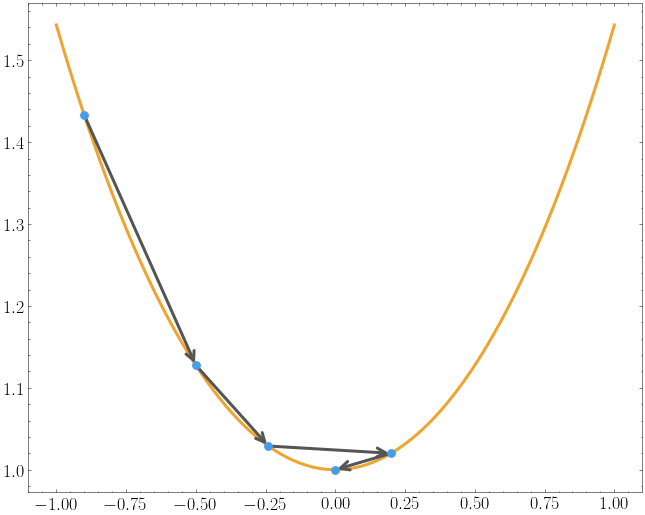
\includegraphics[width=7cm]{images/state-of-art/gradient-descent/gradient.png}
    \caption{Graphical example of the iteration of the descent of the gradient.}
    \label{fig:gradient_descent}
\end{figure}


The terrain in this metaphor would be the function of cost. The person is the value calculated by the cost function, which we want to minimise and therefore we evaluate the slope or gradient only at that point and in that way we do not depend on the derivative of the cost function but on the partial derivative with respect to each of the input values in the neuron. The number of steps that the person will descend is a value known as the \acrlong{lr} and is one more parameter of the neuronal network.
\newline

In figure \ref{fig:gradient_descent}, there are two axes, representing a neuron that has only one input argument. The ordinate axis represents the error of the neuron. A two-dimensional space has been represented, but any dimension can be used since the number of inputs of the neuron is not limited. Using a three-dimensional space, the cost function would be an irregular surface. In fact, the vector $\nabla f$ will always have at least two values, a weight $w$ and the bias $b$.
\newline

This paper does not explain how to calculate the derivative of a function or partial derivative ($\sigma$). That said, mathematically, the process of this algorithm is as follows:

\begin{enumerate}
\item 1.	The $w$ and bias $b$ weights of the neuron want to be adjusted randomly:
\begin{equation}
    ~N(0, \sigma_2)
\end{equation}

\item A loop is made until convergence::
\begin{enumerate}

\item Partial derivatives are calculated for each of the parameters. A partial derivative measure how much impact a single input variable has on the output of the function and is calculated in the same way as a derivative, the only thing that the derivative repeats for each input variable. Each of these values will indicate what is the slope on the axis of that parameter related to
a single input value.


\begin{equation}
    \begin{split}
    \nabla f &= \nabla f_b \oplus \nabla f_w \\\
    \nabla f_b &= \begin{pmatrix} \frac{\partial c}{\partial b} \end{pmatrix}\\
    \nabla f_w &= \begin{pmatrix} \frac{\partial c}{\partial w_1}, & \frac{\partial c}{\partial w_2}, & \cdots , &  \frac{\partial c}{\partial w_n} \end{pmatrix}
  \end{split}
  \label{eqn:gradients}
\end{equation}


Together all the directions, that is, all the partial derivatives form a vector that indicates the direction in which the slope is rising, this vector is also known as a gradient($\nabla f$) and it will have the same number of elements as the input vector and each value will contain the solution to the partial derivative with respect to each of the input values.
\newline

The objective of this function is to minimize and not maximize, so the gradient will be denied indicating the direction in which the slope is descending.

\begin{equation}
    \nabla f = -\nabla f_b \oplus \nabla f_w
\end{equation}

\item The weights are updated with the new values of the negative gradient multiplied by the learning rate. The learning rate is simply a value that determines how large the step will be in each iteration which will be discussed in more detail in section \ref{learningrate}:

\begin{equation}
    \begin{split}
    b^* = b - \eta * \nabla f_b \\
    w^* = w - \eta * \nabla f_w
    \end{split}
\end{equation}

As with the feed-forward algorithm, the descent of the gradient will work in layers, so this last step should be represented as follows::

\begin{equation}
    W^* = W - \eta * \nabla f
\end{equation}

This equation represents that the weights of all the neurons in a layer will be updated.

\end{enumerate}
\end{enumerate}

This method will be applied to all the neurons in the network. Given an error, the descent of the gradient will obtain a vector containing the derivative of the parameters with respect to the cost. That is to say, the gradient will be a vector with different values, the larger this value is, the more correction must be applied to the corresponding parameter. Seen graphically it can be seen in the following way:

\begin{figure}[H]
    \centering
    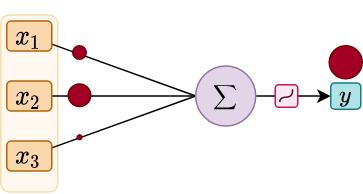
\includegraphics[width=7cm]{images/state-of-art/gradient-descent/gradient_diagram.png}
    \caption{Representation of the descent of the gradient in a neuron The red is the representation of the error.}
    \label{fig:gradient_descent}
\end{figure}

The partial derivatives that must be solved to obtain the gradient vector $\nabla f$, indicates how the cost varies when the parameters $w$ and $b$ are changed. An image of the different parts of the partial derivatives is shown below:


\begin{figure}[H]
    \centering
    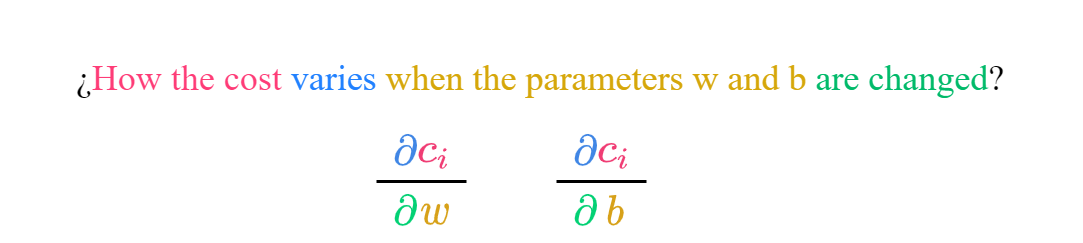
\includegraphics[width=13cm]{images/state-of-art/gradient-descent/dx.png}
    \caption{Partial derivatives used in the descent of the gradient.}
    \label{fig:gradient_descent}
\end{figure}

\end{itemize}


